\documentclass[12pt]{article}

\usepackage{amssymb,amsmath,amsfonts,eurosym,geometry,ulem,graphicx,caption,color,setspace,sectsty,comment,footmisc,caption,natbib,pdflscape,array,hyperref,subcaption}

\usepackage{booktabs}
\usepackage{multirow}



\normalem

\onehalfspacing
\newtheorem{theorem}{Theorem}
\newtheorem{corollary}[theorem]{Corollary}
\newtheorem{proposition}{Proposition}
\newenvironment{proof}[1][Proof]{\noindent\textbf{#1.} }{\ \rule{0.5em}{0.5em}}

\newtheorem{hyp}{Hypothesis}
\newtheorem{subhyp}{Hypothesis}[hyp]
\renewcommand{\thesubhyp}{\thehyp\alph{subhyp}}

\newcommand{\red}[1]{{\color{red} #1}}
\newcommand{\blue}[1]{{\color{blue} #1}}

\newcolumntype{L}[1]{>{\raggedright\let\newline\\arraybackslash\hspace{0pt}}m{#1}}
\newcolumntype{C}[1]{>{\centering\let\newline\\arraybackslash\hspace{0pt}}m{#1}}
\newcolumntype{R}[1]{>{\raggedleft\let\newline\\arraybackslash\hspace{0pt}}m{#1}}

\geometry{left=1.0in,right=1.0in,top=1.0in,bottom=1.0in}

\begin{document}

\begin{titlepage}
\title{The Black Physician Pipeline: \\ Evidence from Medical School Records}
% \title{The Black Physician Pipeline: \\ Evidence from 1979-2020}
\author{Frina Lin\thanks{Email: frina.f.lin@gmail.com. }}
% This work was supported in part by the National Science Foundation Graduate Research Fellowship Program. I thank my advisors David Cutler, Marcella Alsan, and Will Dobbie for their guidance and support and Joseph Doyle and John Graves for sharing code. I thank Mark Shepard, Helen Ho, Grace McCormack, Dayea Oh, and participants at the Harvard Public Economics/Labor Lunch and Health Care Policy seminars for helpful comments. Views are my own.
% as well as Joseph Doyle, Helen Ho, Grace McCormack, Dayea Oh, Mark Shepard.
%\author{Hyunwoo Park\thanks{abc} \and John Smith\thanks{abc}}
\date{August 2, 2022}
\maketitle
\begin{abstract} 

   I show the limited progress in outcomes of Black medical school applicants over the years 1979-2020. Black applicants have grown to 10\% of the applicant pool in recent years, but acceptance rates remain below those of white and Asian applicants. For Black students who do matriculate to medical school, graduation rates lag behind those of white and Asian medical students. Among the cohorts of graduated MDs, medical schools affiliated with historically Black colleges and universities (HBCUs) continue to play an important role in graduating Black physicians, accounting for 14.9\% of Black physicians in 1984-1999 and 14.7\% in 2000-2015. Taken together, the evidence highlights continuing gaps for Black students in the physician pipeline, with need for targeted actions.
\\
\vspace{0in}\\
%\noindent\textbf{Keywords:} key1, key2, key3\\
\vspace{0in}\\
%\noindent\textbf{JEL Codes:} key1, key2, key3\\

\bigskip
\end{abstract}
\setcounter{page}{0}
\thispagestyle{empty}
\end{titlepage}
\pagebreak \newpage


\doublespacing


\section{Introduction} \label{sec:introduction}

Black Americans make up 14.2\% of the population but only 5.3\% of active physicians \citep{aamc_2021_2022}. This underrepresentation mirrors patterns in many high-income careers, including science, engineering, law, and management occupations \citep{wilson_racial_2021}. Given the history of oppression of African Americans in the U.S., the continued underrepresentation of Black Americans in high-status and high-income professions is a cause for examination. In patricular, it is important to critically examine the barriers that Black individuals face in such career pipelines in order to identify external factors which may contribute to underrepresentation today. 

In this paper, I focus on the physician pipeline and document trends in the outcomes of Black medical school applicants, from 1979 through 2020. Using data on applicant, enrollee, and graduation cohorts by race/ethnicity from the Association of American Medical Colleges (AAMC), I find evidence of stagnancy in the graduation of Black doctors. Although the number of Black medical students has increased, particularly in recent years since 2016, acceptance rates and graduation rates for Black students remain below those of white and Asian peers and have stayed relatively constant over the past 40 years. 

Despite the general stagnancy in acceptance rates and graduation rates, I show that there were periods of change. In the mid-1990s, at the height of advocacy for affirmative action, acceptance rates to medical school for Black applicants equaled and even surpassed those of white and Asian applicants. However by the mid-2000s the difference in acceptance rates re-emerged and persisted over the following decades. 

Throughout these periods of change, the graduation rate differential between Black and white students remained constant. Therefore, although acceptance rates varied, there was no evidence of a change in the relative quality of admitted students by race. Black students who were admitted during the height of affirmative action were no less likely to graduate than Black students admitted in earlier or later periods. 

However, the persistent Black-white graduation rate gap suggests that, without external forces, medical schools interested in maintaining high graduation rates may choose to admit fewer Black students. It follows that the schools that have been instrumental to producing Black physicians are those with health care diversity and Black education in their mission, including medical schools affiliated with Historically Black Colleges and Universities (HBCUs): Howard University College of Medicine, Meharry Medical College, and Morehouse School of Medicine. These three schools are just as important to the graduation of Black physicians today as they were in the 1980s. 

This paper contributes to existing work on the role of medical schools in influencing physician diversity. In particular, the AAMC has advocated for and evaluated the success of efforts to improve minority representation in medicine over several decades. In 1991, it launched a 10-year plan with the goal of enrolling a class with 3,000 students from underrepresented minorities by the year 2000 \citep{cohen_case_2002}. This initiative appeared to see immediate results but was hindered by attacks on affirmative action that began in the late-1990s \citep{garces_racial_2015,mickey-pabello_addressing_2018}. My results support this narrative of progress and reversal, while extending the time series to recent years and exploring connections to acceptance rates and graduation rates.  

This work also relates to a growing literature on the importance of physician diversity from a public health perspective. Having a same-race doctor has been found to improve primary care and hospital outcomes for Black patients \citep{alsan_does_2019,hill_physician-patient_2020}. Black physicians are more likely to practice in underserved areas and communities with high percentages of Black residents and, controlling for the racial makeup of the community, care for significantly more Black patients, including more patients covered by Medicaid \citep{komaromy_role_1996, laditka_physician_2004,xierali_racial_2018}. More broadly, diversity in the health care workforce can improve the breadth and depth of the U.S. health research agenda and expand the pool of medically trained individuals who may take up leadership positions in the health care system.






%In order to ensure equal opportunity and access to the range of professions, including the status and income that come with certain professions, it is important to understand the pipeline and the nature of barriers along the way.  

%In an equitable society, we would like to ensure equal opportunity and access to the range of professions, and the status and income that come with certain professions. Beyond this, physician diversity can improve health of the general population, in research as well as treatment and information traveling through networks of family and friends. 

%  Inauguration of the AAMC's Project 3000 by 2000 in 1990, coincided with uptake in admissions of underrepresented minorities. Perhaps the project led to greater effort within existing affirmative action programs. The project also focused on improving equity in access to primary and secondary educational opportunities for low-income minority students, to improve the pipeline to college. The Supreme Court decision in Regents of the University of California v. Bakke in 1978 allowed schools to take race into account in admissions decisions, but came under attack in 1996 in Texas, Mississippi, Louisiana, and California. Medical school enrollment of individuals from minority groups underrepresented in medicine (African Americans, Mexican Americans, Native Americans, and mainland Puerto Ricans) declined since 1996. 

% Many challenges within the broader physician pipeline for Black students (cite Gonzalez 2002)

% Need to support Black medical schools, dedicated to primarily training African American physicians. (cite Harley 2006)



% Paper does not address what happens before and after medical school. (pipeline of math and sciences in college, preparing for and applying to medical school) (pipeline of getting into residency, representation across specialties, obtaining a job and remaining a physician with available patient population.)

% ``Indeed, in medical schools, student body racial diversity is inextricably connected to addressing racial and ethnic health inequities. A racially and ethnically diverse student body leads to more and better prepared doctors who go on to serve communities of color and to more patients of color who seek out care, a first step for receiving it. Research has documented, for example, that relative to their white peers, more doctors of color go on to practice in communities of color, where medical care is already scarce (Komaromy et al. 1996). Empirical research has also shown that minority patients strongly prefer to receive medical care from physicians who share their racial or ethnic background (Saha et al. 2000). Minority patients further rate the quality of their visit more highly when they are treated by a physician of the same race or ethnicity (Saha et al. 1999). And by building cross-cultural competence through exposure to other cultures, languages, and perspectives, a racially diverse student body helps prepare all students to better serve communities of color (Cohen 2003; Guiton et al. 2007; Saha et al. 2008)."

% Race-conscious admissions okay in 1978 U.S. Supreme Court decision in Regents of the University of California v. Bakke.

% Affirmative action bans in California, Washington, Florida, Texas, Michigan, and Nebraska reduced applications modestly with a larger reduction in admissions and enrollments (17\%) of under-represented minorities (Micky-Pabello and Garces 2015, 2018)

% Arizona, new hampshire, and oklahoma, as the implementation of the bans in these states is too recent (2010, 2011, 2012, respectively)

% Texas in 1997
% California as having started in 1997

% Washington (Initiative 200), Florida (one Florida initiative), michigan (proposal 2), and nebraska (initiative 424), which were implemented, respectively, in 1999, 2001, 2007, and 2009

\section{Data and Methods} \label{sec:methods}

\subsection{Data Source}

The data consist of historical tabulations of applicants, matriculants, enrollees, and graduates of U.S. medical schools from the Association of American Medical Colleges (AAMC). In particular, the applicant and matriculant data tables contain annual counts of self-reported race/ethnicity among applicants, acceptees, and matriculants to U.S. medical schools, from application year 1978-1979 through 2019-2020. The enrollment and graduation data tables contain counts of self-reported race/ethnicity separately for each medical school and academic year, from academic year 1979-1980 through 2019-2020. The enrollment data originate from the AAMC Student Records System (SRS).

\subsection{Measurement of Race}

Information on race and ethnicity is collected from multiple AAMC sources including the Medical College Admission Test (MCAT), the American Medical College Application Service (AMCAS), and the Electronic Residency Application Service (ERAS). However, the methodology for collecting data on race/ethnicity has changed over time. Prior to academic year 2002-2003, an individual could identify with one and only one race/ethnicity category, whereas starting from academic year 2002-2003 individuals could select multiple race categories. In the analysis, I include individuals who have designated multiple races/ethniticies in  each of the race/ethnicity categories that were selected.

In relevant figures, I include a dashed line to highlight the year after which individuals could designate multiple races. 

\subsection{Estimation of Graduation Rates}\label{sec:gradrate}

I construct approximate graduation rates. For each year $t$, race $r$, and medical school $m$, I observe student enrollment $E$ across all four years, as well as the number of graduates $G$ in the given year. I do not observe enrollment numbers for any specific graduating class. I therefore estimate graduation rates $g$ as follows: 
\begin{align}
g_{t-1.5,r,m} = \frac{\sum_t^{t+3} G_{trm}}{E_{trm}}.
\end{align}
For example, for the 1984-1985 enrolled class, I compute the number of graduates observed in 1985, 1986, 1987, and 1988 as the numerator. I assign this graduation rate to year $t-1.5 = 1982.5$, because it represents graduates from matriculation years 1981, 1982, 1983, and 1984. Broadly, this is similar to a 4-year graduation rate, but because I do not have enrollment counts for specific graduating classes some students could take more time and still be included as graduating.


\section{Results and Discussion} \label{sec:results}

I begin by showing trends in the number of applicants to medical schools over the years 1979-2020. The number of applicants has fluctuated widely, reaching a low of 26,709 applicants in 1989, a peak of 46,965 applicants in 1997, and growing steadily since 2004 to a high of 53,371 applicants in 2020 (Figure \ref{fig:app_total}). The same qualitative patterns in applicant counts are present among Black applicants (Figure \ref{fig:app_black}), as well as across other observable subgroups, including first-time applicants, white applicants, and Asian applicants. 

Despite ebbs and flows in the number of applicants, Figure \ref{fig:app_total} shows that the total number of accepted and matriculated medical students remained relatively consistent, before growing slowly since 2005. In contrast, there are a few noticeable patterns in the number of Black accepted and matriculated students over the observed time period (Figure \ref{fig:app_black}). In particular, the mid-1990s saw an increase in the number of Black accepted and matriculated students, from 992 matriculated students in 1989 to a peak of 1,309 matriculants in 1995. However, this increase was short-lived, decreasing back down to 1,131 matriculants by 2000 and remaining relatively steady for the following decade. Since then, there has been a notable increase in Black accepted and matriculated students starting in 2016, corresponding with a sharp increase in the number of applicants.

To contextualize the variation in the number of Black matriculants in terms of the racial composition of medical students, Figure \ref{fig:app_blackshare} shows the \textit{share} of applicants and matriculants who identify as Black over the study period. We see that the Black applicant share has grown slowly over time, from 6.6 percent of the applicant pool in 1979 to 9.7 percent in 2020, but still remains below the population share of 14.2 percent in 2020 \citep{jones_2020_2021}. In addition, the Black matriculant share has consistently been below the Black applicant share, by about 1pp, with the exception of the mid-1990s, when Black students made up about 8 percent of both total applicants and matriculants. 

From the perspective of an individual Black applicant, the convergence of Black applicant and matriculant shares in the mid-1990s suggests that acceptance rates may have increased for Black applicants during this period. However, Figure \ref{fig:acceptance} shows that acceptance rates for Black applicants have remained relatively consistent over the study period, varying between a high of 50 percent in 1990 and a low of 35 percent in 2016. Acceptance rates for white and Asian medical school applicants have fluctuated more widely, between highs of 67 percent and 66 percent respectively in 1989 and lows of 38 percent and 34 percent respectively in 1996. In particular, acceptance rates for white and Asian applicants dipped in the mid-1990s to equal and fall below those of Black applicants. By the mid-2000s, acceptance rates for white and Asian students diverged from those of Black applicants again, remaining more than 5pp above acceptance rates for Black applicants in recent years.

The difference in acceptance rates could reflect overall differences in the quality of applicants, as admissions committees take into consideration many factors including GPAs, MCAT scores, volunteer work, and research when selecting applicants. To investigate whether differences in applicant quality may explain the persistent Black-white differential in acceptance rates, I plot an observable metric of student quality: graduation rates. 

In Figure \ref{fig:graduation} I show that Black medical students across the study period had lower graduation rates than white and Asian students. However, I do not observe any differential trends in graduation rates for Black students relative to white and Asian students, while the acceptance rate differential widened, closed, and reemerged again. The graduation rate for Black medical students remained steadily around 81 percent in the 1980s and 1990s, before increasing to 83 percent with the composition change once students could designate multiple races. The consistency of the Black-white graduation rate gap, as admissions policies varied, suggests that there is limited scope on the margin for selection of applicants who are more likely to be successful, within race. 

On the other hand, the persistent Black-white graduation rate gap, which averaged 9.6 percentage points across years, does provide an explanation for lagging acceptance rates among Black applicants. If medical schools aim to improve their graduation rates, they may accept fewer Black students who may be statistically less likely to graduate. Further, the gap is not driven by sorting across schools: controlling for medical school the Black-white graduation rate gap remains at 10.4 percentage points.

Given the challenges in admitting and graduating Black medical students, I turn to examine the most successful educators of Black physicians during the study period. Table \ref{tab:top10} shows that medical schools affiliated with Historically Black Colleges and Universities (HBCUs) have played and continue to play a very important role in educating Black physicians. Howard University College of Medicine in D.C., Meharry Medical College in Nashville, TN, and Morehouse School of Medicine in Atlanta, GA were among the top 5 medical schools producing Black MDs in graduating years 1984-1999, and became the top 3 in 2000-2015. Together, these schools graduated nearly 15\% of Black physicians both in 1984-1999 and in 2000-2015, through student cohorts with very high Black student shares of 60-80 percent. 

In addition, other schools that have graduated many Black MDs include the University of Illinois College of Medicine in Chicago, IL, Wayne State University School of Medicine in Detroit, MI, SUNY Downstate Medical Center College of Medicine in Brooklyn, NY, and the UNC School of Medicine in Chapel Hill, NC. In contrast to the HBCU-affiliated medical schools, these tend to be large medical schools with Black student shares ranging from 7-11 percent.  

\subsection{Implications for Practice and Policy}

%I have documented stagnancy in acceptance rates and graduation rates among Black medical school candidates. (highlight what is new relative to literature). In this section, I address implications of and limitations to these results, which provide opportunities for further research. 

%\subsection{Statistical Discrimination}

The results show that, despite ongoing discussions about physician diversity in research and policy spheres, there has been marked stagnancy in achieving meaningful increases in newly graduated physicians from underrepresented groups. In particular, I highlight the Black-white graduation rate gap and its implications for admissions as a potential roadblock in efforts to increase Black enrollment in and graduation from medical schools. In response, policy levers that improve graduation rates of Black medical students, such as ensuring social, academic, and financial support during medical school as well as maintaining partnerships with K-12 education systems and colleges to strengthen preparedness, could in turn lead to higher acceptance rates at the admissions stage. Future research should seek to understand barriers facing Black medical students that lead to lower graduation rates.

On the other hand, given recent research regarding public health benefits of Black physicians for marginalized Black communities, we may believe that the societal impact of training more Black doctors is important enough that greater admissions despite lower graduation rates could be rationalized for Black students. In this case, an external actor beyond individual medical school interests would be required. To align medical school incentives, we may want to develop an ``impact factor" to measure and rank public health impacts of medical schools beyond standard metrics such as graduation rates. Because of the divergence of interests, HBCUs and other schools with health care equity and physician diversity in their mission remain crucial for the education of Black doctors, and need to be supported if we hope to develop a more diverse physician workforce.


\subsection{Limitations}

This study has several limitations. First, the analysis and conclusions are based on aggregate time trends, and do not control for individual characteristics of applicants such as GPA, MCAT scores, courses taken, and demographic characteristics beyond race. Therefore, the relationships between applicant counts, acceptance rates, and graduation rates are suggestive and should not be interpreted as causally linked. Unmeasured social and economic confounders that shift over time may affect all documented series. Although the correlational analysis in this study cannot demonstrate causal mechanisms, it is a step toward determining which factors are likely to contribute to underrepresentation of Black Americans among physicians. 

Second, this paper focuses solely on outcomes for students between application and graduation from US medical schools granting MD degrees. I do not observe data on other health care professions and degrees, such as DO, physician assistant, and nursing programs, which Black students may opt into with or without applying to MD-granting medical schools. These other degrees may act as substitutes for or complements to the graduation of Black physicians with MD degrees and their presence can affect the diversity of the health care workforce from the patient's perspective. Nevertheless, of these degrees, MD credentials generate the highest incomes and decision-making power and are therefore important to study to improve diversity and equity at the highest levels. 

Finally, I do not observe data on portions of the physician pipeline before and after medical school, including K-12 and college education, medical specialty decisions, residency, and professional practice following medical school. These inputs and decision points represent many additional opportunities for intervention and potential challenges that deeply affect the overall idea of reaching close to parity between Black population and Black physician shares. However, documenting disparities within the medical school application and graduation process is a step towards understanding challenges within the full pipeline. 

\section{Conclusion}

I show stagnancy in acceptance rates, graduation rates, and number of graduates among Black medical school applicants over the years 1979-2020. These results highlight challenges in the pipeline for Black physicians and the continuing role of mission-driven institutions in training and graduating Black doctors. 

% \begin{quote}
%   ``You may never know what results come of your action, but if you do nothing there will be no result."
%   \flushright{-- Mahatma Gandhi}
% \end{quote}

\clearpage

\singlespacing
\setlength\bibsep{6pt}
\bibliographystyle{aer}
\bibliography{dissertation2022}




\clearpage

\onehalfspacing

\addcontentsline{toc}{section}{Tables}


\clearpage

\addcontentsline{toc}{section}{Figures}

\begin{figure}[hp]
 \centering
 \caption{Applicants, Acceptees, and Matriculants, 1979-2020}
 \label{fig:app}
 \begin{subfigure}{0.9\textwidth}
  \centering
  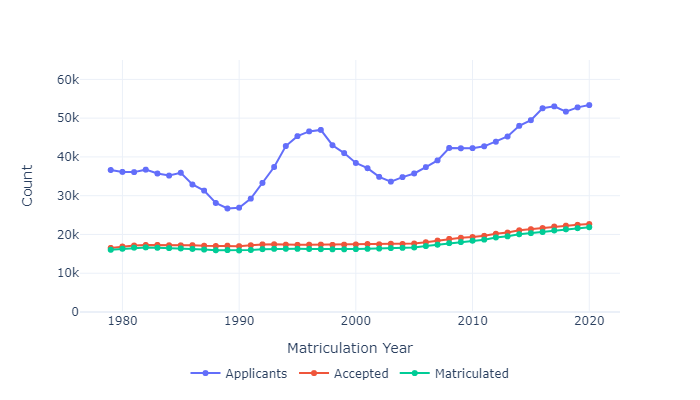
\includegraphics[width=\textwidth]{figs/applicant_count_total.png}
  \caption{Total}
  \label{fig:app_total}
\end{subfigure}
 \begin{subfigure}{0.9\textwidth}
   \centering
   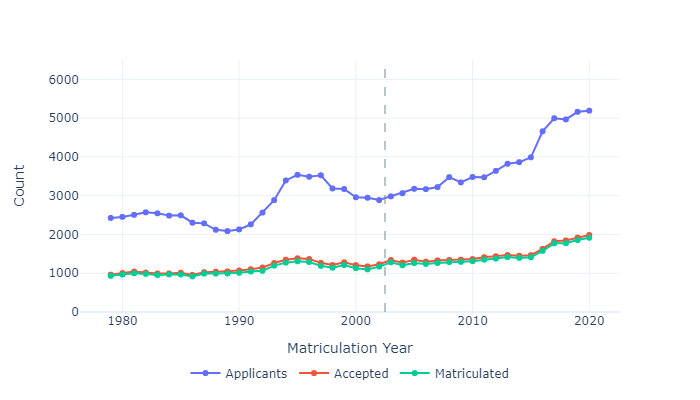
\includegraphics[width=\textwidth]{figs/applicant_count_black.png}
   \caption{Black}
   \label{fig:app_black}
 \end{subfigure} 
      \begin{minipage}{0.9\textwidth}
      \footnotesize Notes: Data are from the AAMC Applicant and Matriculant Data File. Panel A shows the total number of applicants, acceptees, and matriculants to U.S. medical schools for academic years 1979-1980 through 2020-2021. Panel B shows the number of applicants, acceptees, and matriculants who self-identified as Black or African American. Prior to matriculation year 2003-2004, individuals could identify with one and only one race/ethnicity. The dashed line indicates the year after which individuals could designate multiple races. 
      \end{minipage}
\end{figure}


\begin{figure}[hp]
   \centering
   \caption{Black Share of Applicants and Matriculants, 1979-2020}
   \label{fig:app_blackshare}
   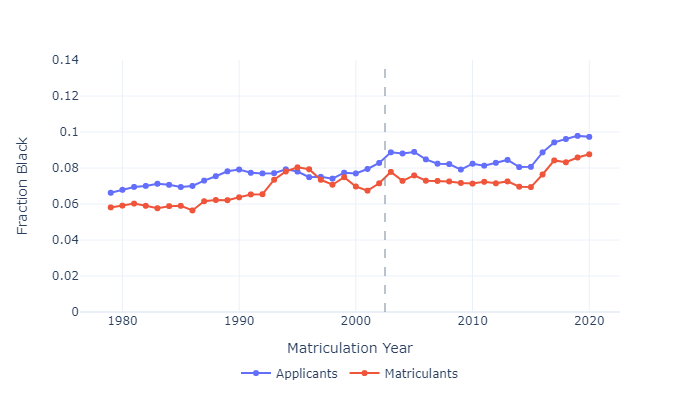
\includegraphics[width=\textwidth]{figs/matriculant_frac_black.png}
   \begin{minipage}{0.9\textwidth}
   \footnotesize Notes: Data are from the AAMC Applicant and Matriculant Data File. The series show the number of applicants and matriculants to U.S. medical schools who self-identified as Black or African American divided by the total number of applicants and matriculants for each academic year, from 1979-1980 through 2020-2021. Prior to matriculation year 2003-2004, individuals could identify with one and only one race/ethnicity. The dashed line indicates the year after which individuals could designate multiple races. 
   \end{minipage}
  \end{figure}


  \begin{figure}[hp]
   \centering
   \caption{Acceptance Rates by Race, 1979-2020}
   \label{fig:acceptance}
   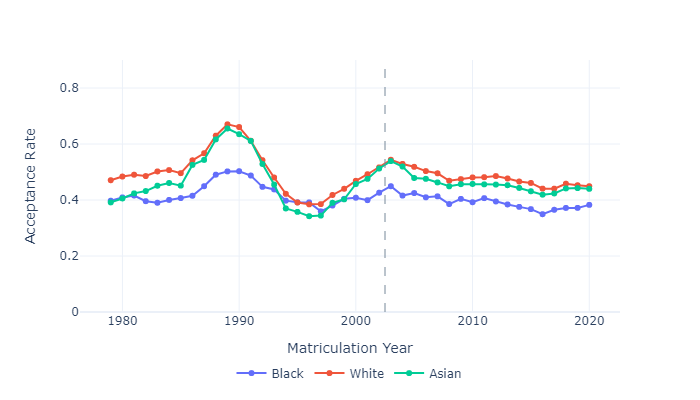
\includegraphics[width=\textwidth]{figs/acceptance_rate_byrace.png}
   \begin{minipage}{0.9\textwidth}
   \footnotesize Notes: Data are from the AAMC Applicant and Matriculant Data File. The series show the number of acceptees divided by the number of applicants to U.S. medical schools by race, for individuals who self-identified as Black or African American, White, and Asian. Prior to matriculation year 2003-2004, individuals could identify with one and only one race/ethnicity. The dashed line indicates the year after which individuals could designate multiple races. 
   \end{minipage}
  \end{figure}

  \begin{figure}[hp]
    \centering
    \caption{Graduation Rates by Race, 1980-2015}
    \label{fig:graduation}
    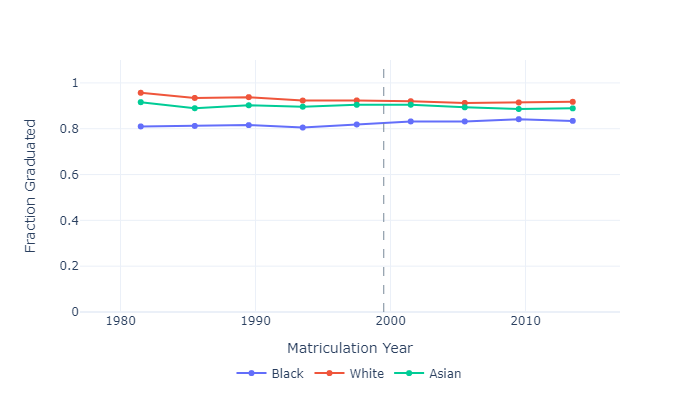
\includegraphics[width=\textwidth]{figs/gradrate_byrace.png}
    \begin{minipage}{0.9\textwidth}
    \footnotesize Notes: Data are from the AAMC Student Records System (SRS). The series show estimated graduation rates as described in Section \ref{sec:gradrate}, for students who self-identified as Black or African American, White, and Asian. Prior to academic year 2002-2003, individuals could identify with one and only one race/ethnicity. The dashed line indicates the point after which individuals could designate multiple races. The dashed line occurs at an earlier matriculation year because the graduation rates are computed from data collected at a later date. 
    \end{minipage}
   \end{figure}
 

\clearpage
\begin{landscape}
% Please add the following required packages to your document preamble:
% \usepackage{multirow}
\begin{table}[]
  \centering
  \small
  \caption{Top 10 Schools Graduating Black Physicians, 1984-1999 and 2000-2015}
  \label{tab:top10}
  \begin{tabular}{clcccc}
    \hline\hline
    \multirow{2}{*}{} & \multirow{2}{*}{}     & \multirow{2}{*}{\parbox{2cm}{Black \\ Graduates}} & \multirow{2}{*}{\parbox{1.5cm}{Share \\ Black}} & \multirow{2}{*}{\parbox{3.1cm}{Share of Total  \\ Black Graduates}} & \multirow{2}{*}{\parbox{2.2cm}{Graduation \\ Rate}} \\
                        &                                          &                                  &                              &                                                   &                                  \\
                        &  & (1) & (2) & (3) & (4) \\
                        \hline
  \multicolumn{2}{l}{\textbf{A. 1984 -   1999}}                          &                                  &                              &                                                   &                                  \\
  1  & Howard University COM                    & 998  & 0.666 & 0.068 & 0.845 \\
  2  & Meharry Medical College                  & 841  & 0.754 & 0.057 & 0.725 \\
  3  & University of Illinois COM               & 429  & 0.093 & 0.029 & 0.737 \\
  4  & Wayne State University SOM               & 379  & 0.094 & 0.026 & 0.791 \\
  5  & Morehouse SOM                            & 361  & 0.786 & 0.024 & 0.808 \\
  6  & Lewis Katz SOM at Temple University      & 296  & 0.104 & 0.020 & 0.876 \\
  7  & UNC at Chapel Hill SOM                   & 290  & 0.096 & 0.020 & 0.842 \\
  8  & UCLA David Geffen SOM                    & 281  & 0.114 & 0.019 & 0.824 \\
  9  & SUNY Downstate Medical Center COM        & 274  & 0.100 & 0.019 & 0.849 \\
  10 & Rutgers New Jersey Medical School        & 264  & 0.102 & 0.018 & 0.825                   \vspace{2mm} \\ 
  \multicolumn{2}{l}{\textbf{B. 2000 -   2015}}                             &                                  &                              &                                                   &                                  \\
  1  & Meharry Medical College                  & 1052 & 0.659 & 0.059 & 0.842 \\
  2  & Howard University COM                    & 1042 & 0.777 & 0.058 & 0.777 \\
  3  & Morehouse SOM                            & 537  & 0.727 & 0.030 & 0.913 \\
  4  & University of Illinois COM               & 443  & 0.094 & 0.025 & 0.805 \\
  5  & University of Texas Medical Branch SOM   & 361  & 0.087 & 0.020 & 0.717 \\
  6  & Wayne State University SOM               & 348  & 0.110 & 0.019 & 0.983 \\
  7  & SUNY Downstate Medical Center COM        & 326  & 0.100 & 0.018 & 0.905 \\
  8  & UNC at Chapel Hill SOM                   & 289  & 0.115 & 0.016 & 0.778 \\
  9  & Medical University of South Carolina COM & 261  & 0.099 & 0.015 & 0.774 \\
  10 & GWU SOM and Health Sciences              & 258  & 0.066 & 0.014 & 0.837             \\
  \hline \hline       
  \end{tabular}
  \vspace{3mm}

  \begin{minipage}{1.15\textwidth}
    \footnotesize Notes: Data are from the AAMC Student Records System (SRS). Abbreviations are used in school names for College of Medicine (COM) and School of Medicine (SOM). Column (1) reports the cumulative number of graduates who self-identified as Black or African American. Column (2) reports the share of graduates from each school who identified as Black. Column (3) reports the share of total Black graduates from the period accounted for by a specific school. Column (4) reports the estimated graduation rate among Black enrollees at each school. Prior to academic year 2002-2003, individuals could identify with one and only one race/ethnicity. Aftwards, individuals could designate multiple races and are included as long as they self-identified as Black. 
    \end{minipage}
  \end{table}

\end{landscape}

\appendix

\setcounter{table}{0}
\renewcommand{\thetable}{A\arabic{table}}

\setcounter{figure}{0}
\renewcommand{\thefigure}{A\arabic{figure}}


\end{document}